\documentclass[a4paper,12pt]{report}
\usepackage{graphicx}
\usepackage{hyperref}
\usepackage{index}
\pagestyle{empty}
\usepackage{geometry}
\usepackage{titlesec}
\usepackage{subcaption}
\usepackage{setspace} % For line spacing
\geometry{margin=1in}
\setcounter{secnumdepth}{0}  % Disable numbering for chapters and sections

\titleformat{\section} % Section formatting
  {\normalfont\Huge\bfseries} % Text format
  {} % Label
  {0pt} % Space between label and title
  {} % Before code

\titleformat{\subsection} % Subsection formatting
  {\normalfont\large\bfseries} % Text format
  {} % Label
  {0pt} % Space between label and title
  {} % Before code

\titlespacing*{\section}
  {0pt}{3.5ex plus 1ex minus .2ex}{2.3ex plus .2ex} % No indentation, standard spacing

\titlespacing*{\subsection}
  {0pt}{1.5ex plus 0.5ex minus .2ex}{0.5ex plus .2ex} % Reduce the space before and after subsection titles

% Reset paragraph indentation for content under subsections
\setlength{\parindent}{40pt}

\newindex{main}{idx}{ind}{Index}

\begin{document}
\setcounter{tocdepth}{1}

% Title Page
\begin{titlepage}
    \centering
    \vspace*{1cm}

    \Huge
    \textbf{University Lab Practical File}\\
    Microelectronic Circuits and Applications
    \newpage 

    
\includegraphics[width=0.4\textwidth]{../Img/NSUT_logo.png}\\[1.5em]
    {\Huge \textbf{CERTIFICATE}}

    \vspace{2cm}

    \raggedright
    \begin{spacing}{1.5}
    \large This is to certify that Mr. / Ms. \underline{\hspace{6cm}} bearing roll no \underline{\hspace{10cm}} of B. Tech \underline{\hspace{4cm}} semester \underline{\hspace{2cm}} of branch \underline{\hspace{8cm}} has satisfactorily completed \underline{\hspace{12cm}} laboratory work during the academic year \underline{\hspace{8cm}}.
    \end{spacing}

    \vfill

    % Signature Section
    \large
% Signature Section
    \noindent
    \begin{minipage}[t]{0.2\textwidth}
        \textbf{Signature of HOD} \\
    \end{minipage}%
    \hfill
    \begin{minipage}[t]{0.2\textwidth}
        \textbf{Signature of Teacher} \\
    \end{minipage}%
    \hfill
    \begin{minipage}[t]{0.2\textwidth}
        \textbf{Signature of Professor} \\
    \end{minipage}


\end{titlepage}

\newpage

% Index
\tableofcontents
\newpage

% Experiment Template

\section{Experiment 1}

  \subsection{Aim:}
    \hspace{20pt}Building a Differential Amplifier

  \vspace{0.3cm} % Adjust spacing between sections

  \subsection{Software Used:} 
    \hspace{20pt}LTSpice

  \vspace{0.3cm}

  \subsection{Design Parameters:}
    \begin{itemize}
        \item CS NMOS W/L = 0.36u/0.18u
        \item CD NMOS W/L = 0.9u/0.18u
    \end{itemize}

  \vspace{0.3cm}

  \subsection{Theory:} 
    \begin{enumerate}
        \item \textbf{Function}: A differential amplifier amplifies the difference between two input signals while rejecting common signals, making it effective in reducing noise or interference.

        \item \textbf{Structure}: It typically uses two transistors with a shared emitter/source. The output is the amplified difference between the inputs, with resistors or current sources setting gain and operating points.

        \item \textbf{Uses}: Differential amplifiers are essential in analog circuits, particularly in operational amplifiers and sensor signal conditioning, where precise signal processing is needed.

    \end{enumerate}

  \vspace{0.3cm}

  \subsection{Circuit Diagram:} 
    \begin{figure}[htbp]
    \centering
      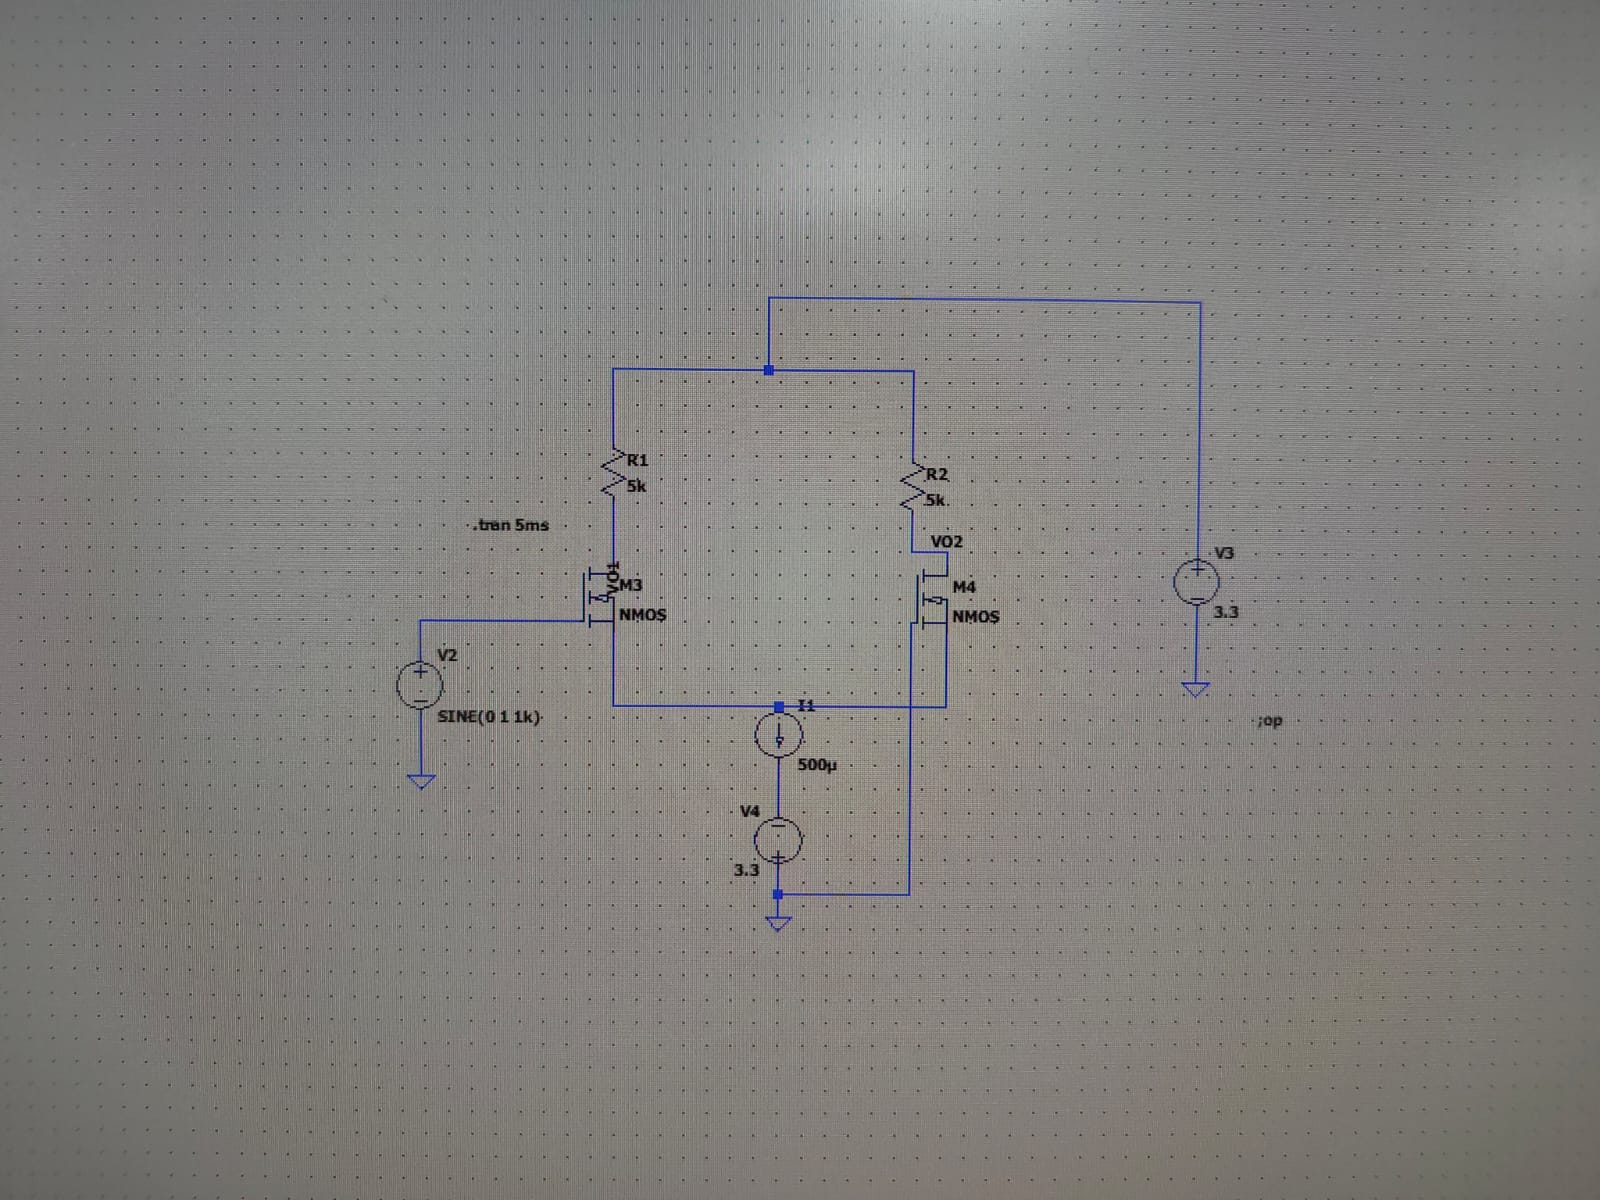
\includegraphics[width=0.5\textwidth]{../Img/E1Ckt.jpeg}
    \caption{Circuit Diagram}
    \label{fig:image}
    \end{figure}

    \vspace*{\fill} % Fills the page with space to ensure that the content stays on a new page
    \newpage

  \subsection{Output:} 
    \begin{figure}[h!]
        \centering
        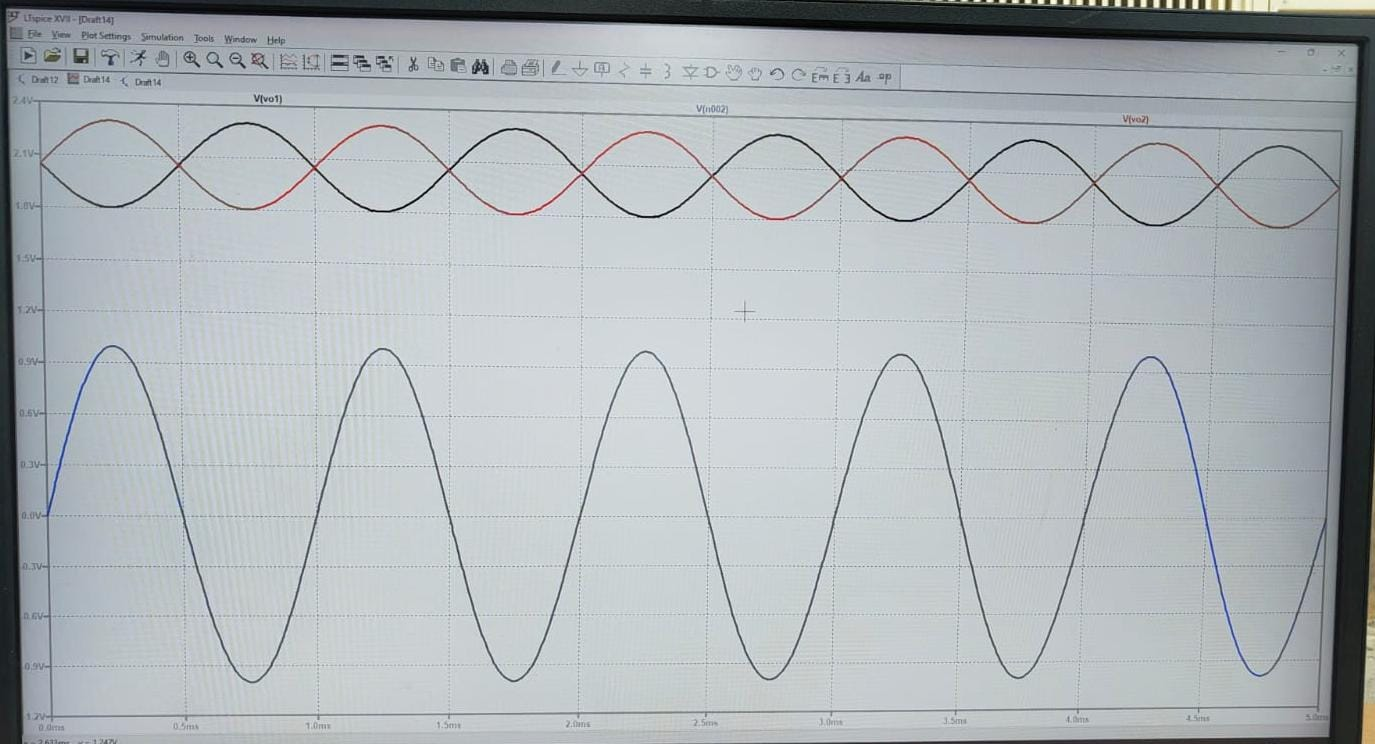
\includegraphics[width=0.8\textwidth]{../Img/E1Tran.jpeg}
        \caption{Output waveform from LTSpice}
    \end{figure}

  \vspace{0.3cm}

  \subsection{Conclusion:} 
    \hspace{20pt}Implemented Differential Amplifier and performed Transient Analysis on it.

  \newpage

\section{Experiment 2}

  \subsection{Aim:}
    \hspace{20pt}Design a Cascode Amplifier

  \vspace{0.3cm}

  \subsection{Software Used:}
    \hspace{20pt}LTSpice 

  \vspace{0.3cm}

  \subsection{Design Parameters:}
    \begin{itemize}
        \item CS NMOS W/L = 0.36u/0.18u
        \item CD NMOS W/L = 0.9u/0.18u
    \end{itemize}

  \vspace{0.3cm}

  \subsection{Theory:} 
    \begin{enumerate}
        \item \textbf{Function}: A cascode amplifier improves gain and bandwidth by stacking two transistors, reducing the Miller effect and enhancing frequency response.

        \item \textbf{Structure}: It consists of a common-emitter/source stage followed by a common-base/gate stage. This configuration boosts gain and isolates input-output interactions.

        \item \textbf{Uses}: Cascode amplifiers are widely used in RF circuits, analog signal processing, and in scenarios where high gain and wide bandwidth are required.
    \end{enumerate}

  \vspace{0.3cm}

  \subsection{Circuit Diagram:} 
  \vspace*{1em}
  \begin{figure}[htbp]
  \centering
    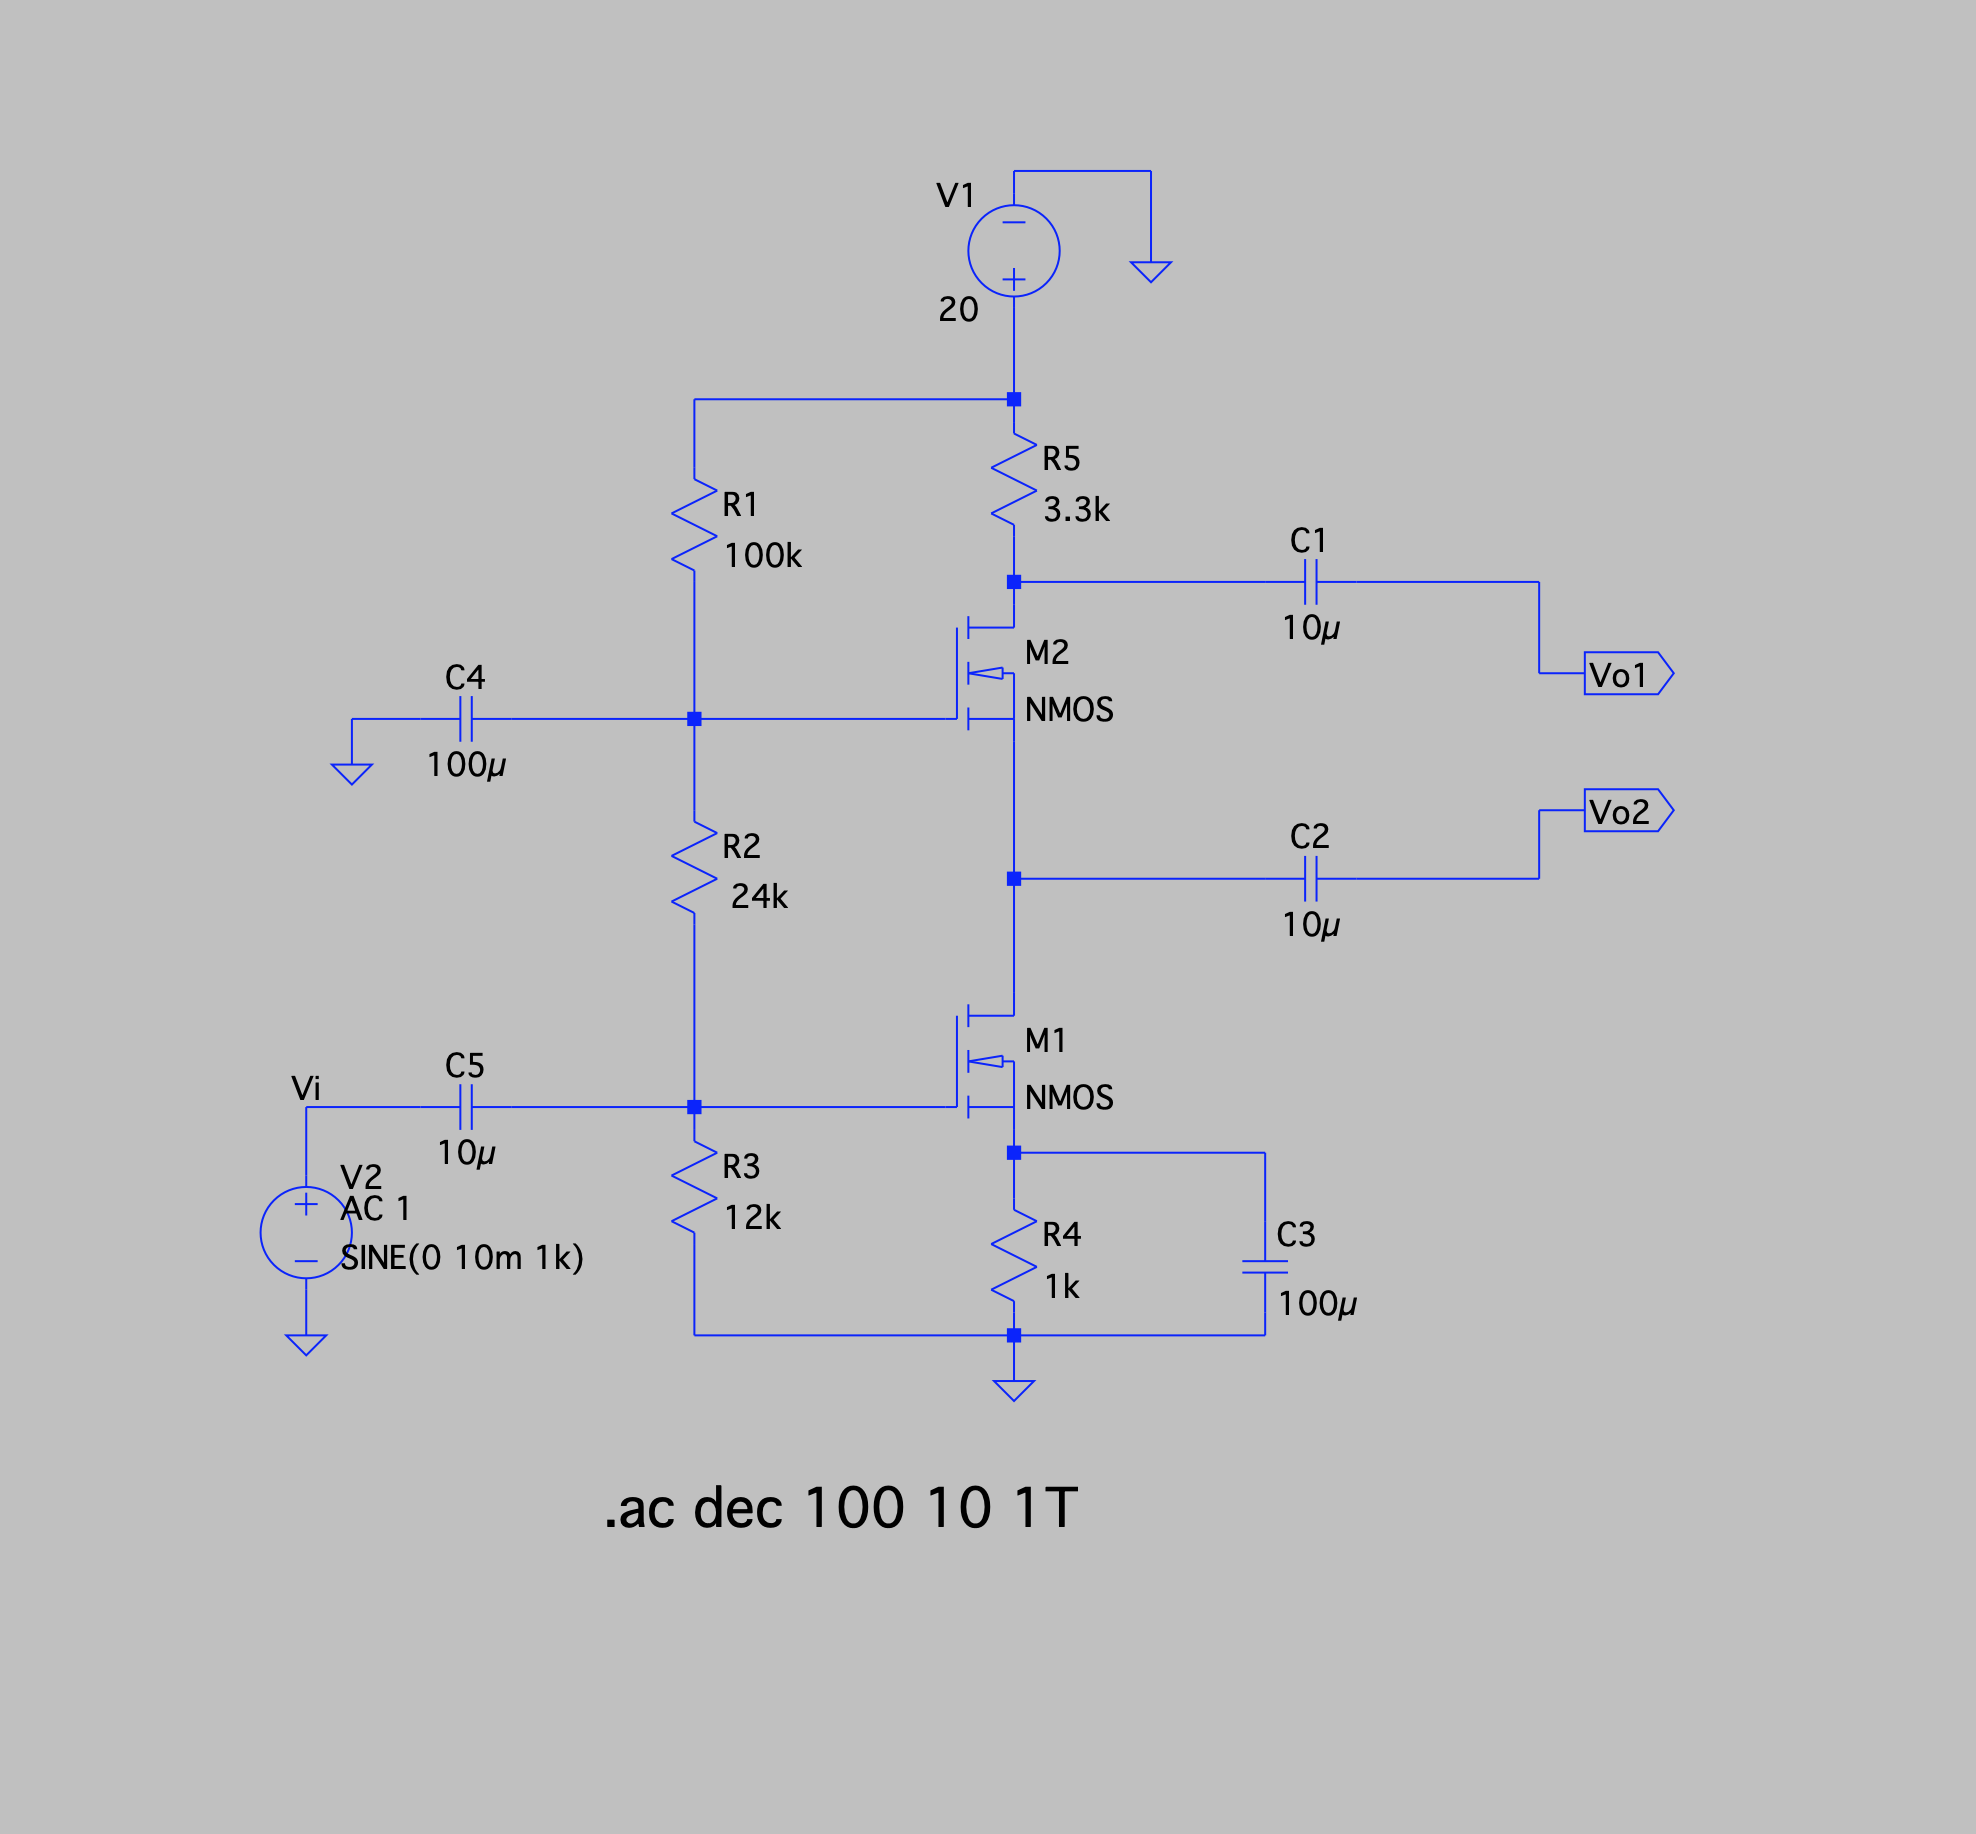
\includegraphics[width=0.5\textwidth]{../Img/E2Ckt.png}
  \caption{Circuit Diagram}
  \label{fig:image}
  \end{figure}

  \vspace*{\fill} % Fills the page with space to ensure that the content stays on a new page
  \newpage

  \subsection{Output:} 
    \hspace{20pt}\begin{figure}[h!]
        \begin{subfigure}[b]{0.48\textwidth} % Adjust the width as needed
        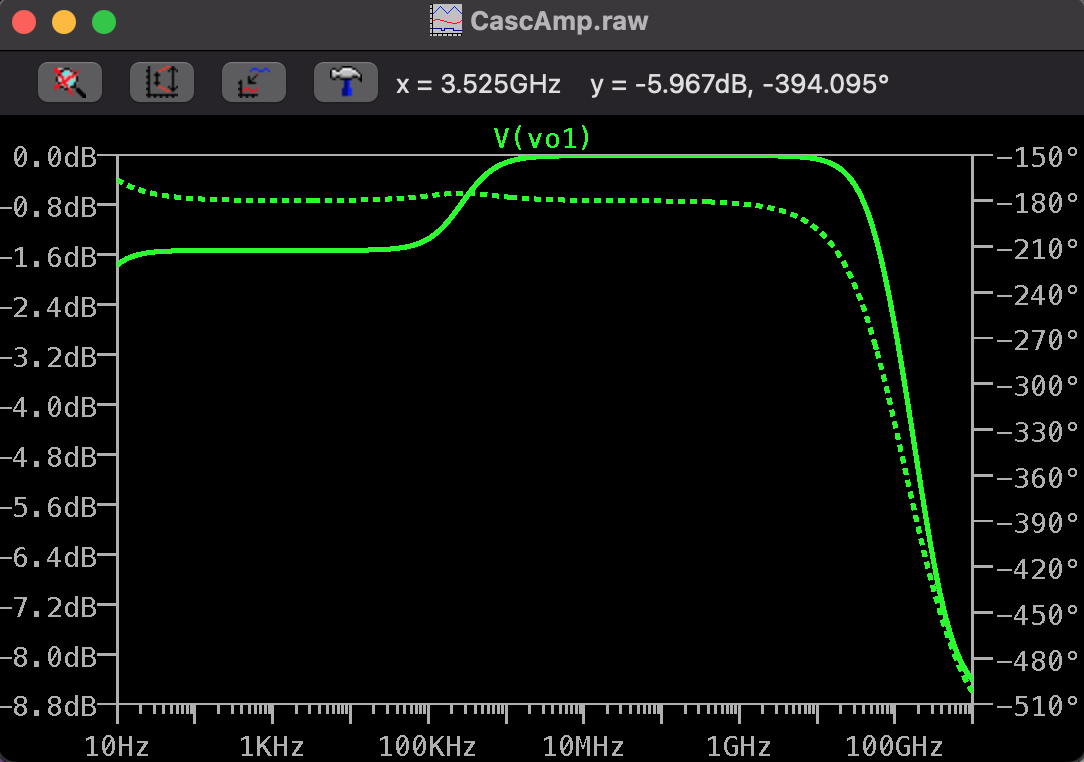
\includegraphics[width=\textwidth]{../Img/E2ACOp.png}
        \caption{AC Analysis Graph with phase}
    \end{subfigure}
    \hfill
    \begin{subfigure}[b]{0.48\textwidth} % Adjust the width as needed
        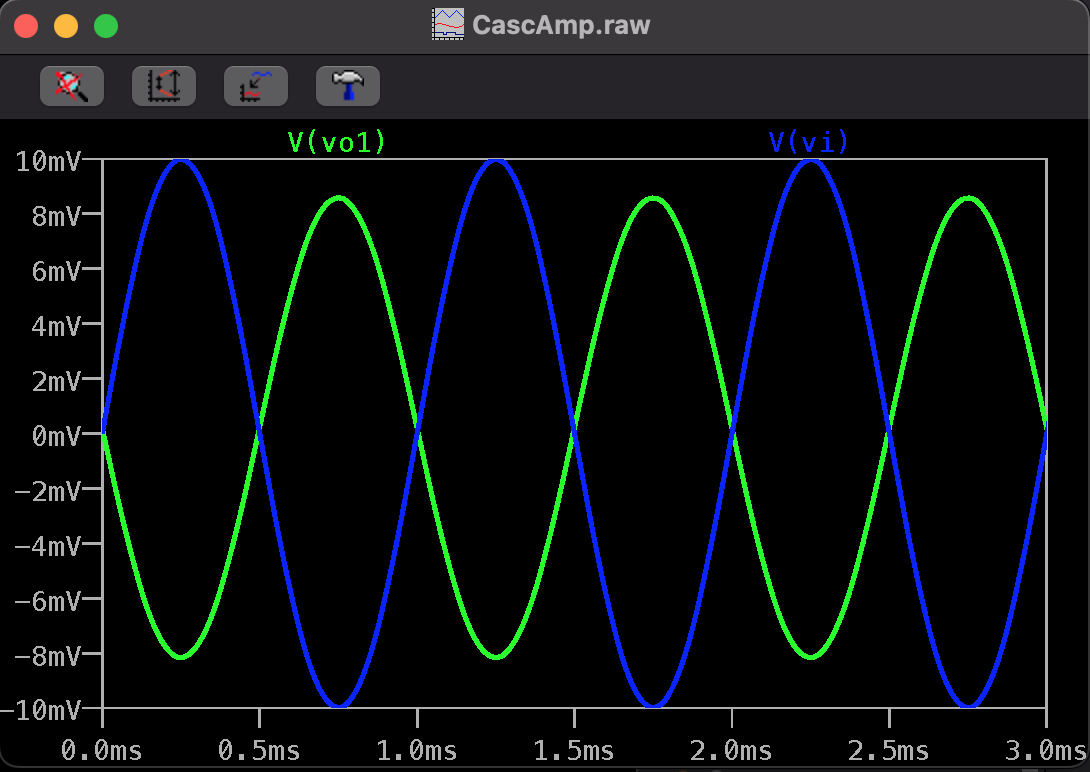
\includegraphics[width=\textwidth]{../Img/E2Tran.png}
        \caption{Transient Analysis Graph}
    \end{subfigure}
    \caption{AC and Transient Analysis Graphs}

    \end{figure}

  \vspace{0.3cm}

  \subsection{Conclusion:} 
    \hspace{20pt}Designed a Cascode Amplifier and performed AC and DC analysis on it.

  \newpage

\section{Experiment 3}

  \subsection{Aim:}
    \hspace{20pt}Building a Basic Triangular wave generator.

  \vspace{0.3cm} % Adjust spacing between sections

  \subsection{Software Used:} 
    \hspace{20pt}LTSpice

  \vspace{0.3cm}

  \subsection{Design Parameters:}
    \begin{itemize}
        \item Opertaional Amplifier OP07
    \end{itemize}

  \vspace{0.3cm}

  \subsection{Theory:} 
    \begin{enumerate}
        \item \textbf{Function}: A triangular wave generator produces a linear, periodic waveform with equal rise and fall times, typically used in waveform generation and modulation.

        \item \textbf{Structure}: The circuit consists of an op-amp configured as an integrator, which converts a square wave input into a triangular output. The square wave is often generated by another op-amp configured as a Schmitt trigger.

        \item \textbf{Uses}: Triangular wave generators are employed in function generators, audio synthesis, and pulse-width modulation (PWM) circuits, where precise waveform generation is needed.
    \end{enumerate}

  \vspace{0.3cm}

  \subsection{Circuit Diagram:} 
  \vspace*{1em}
  \begin{figure}[htbp]
  \centering
    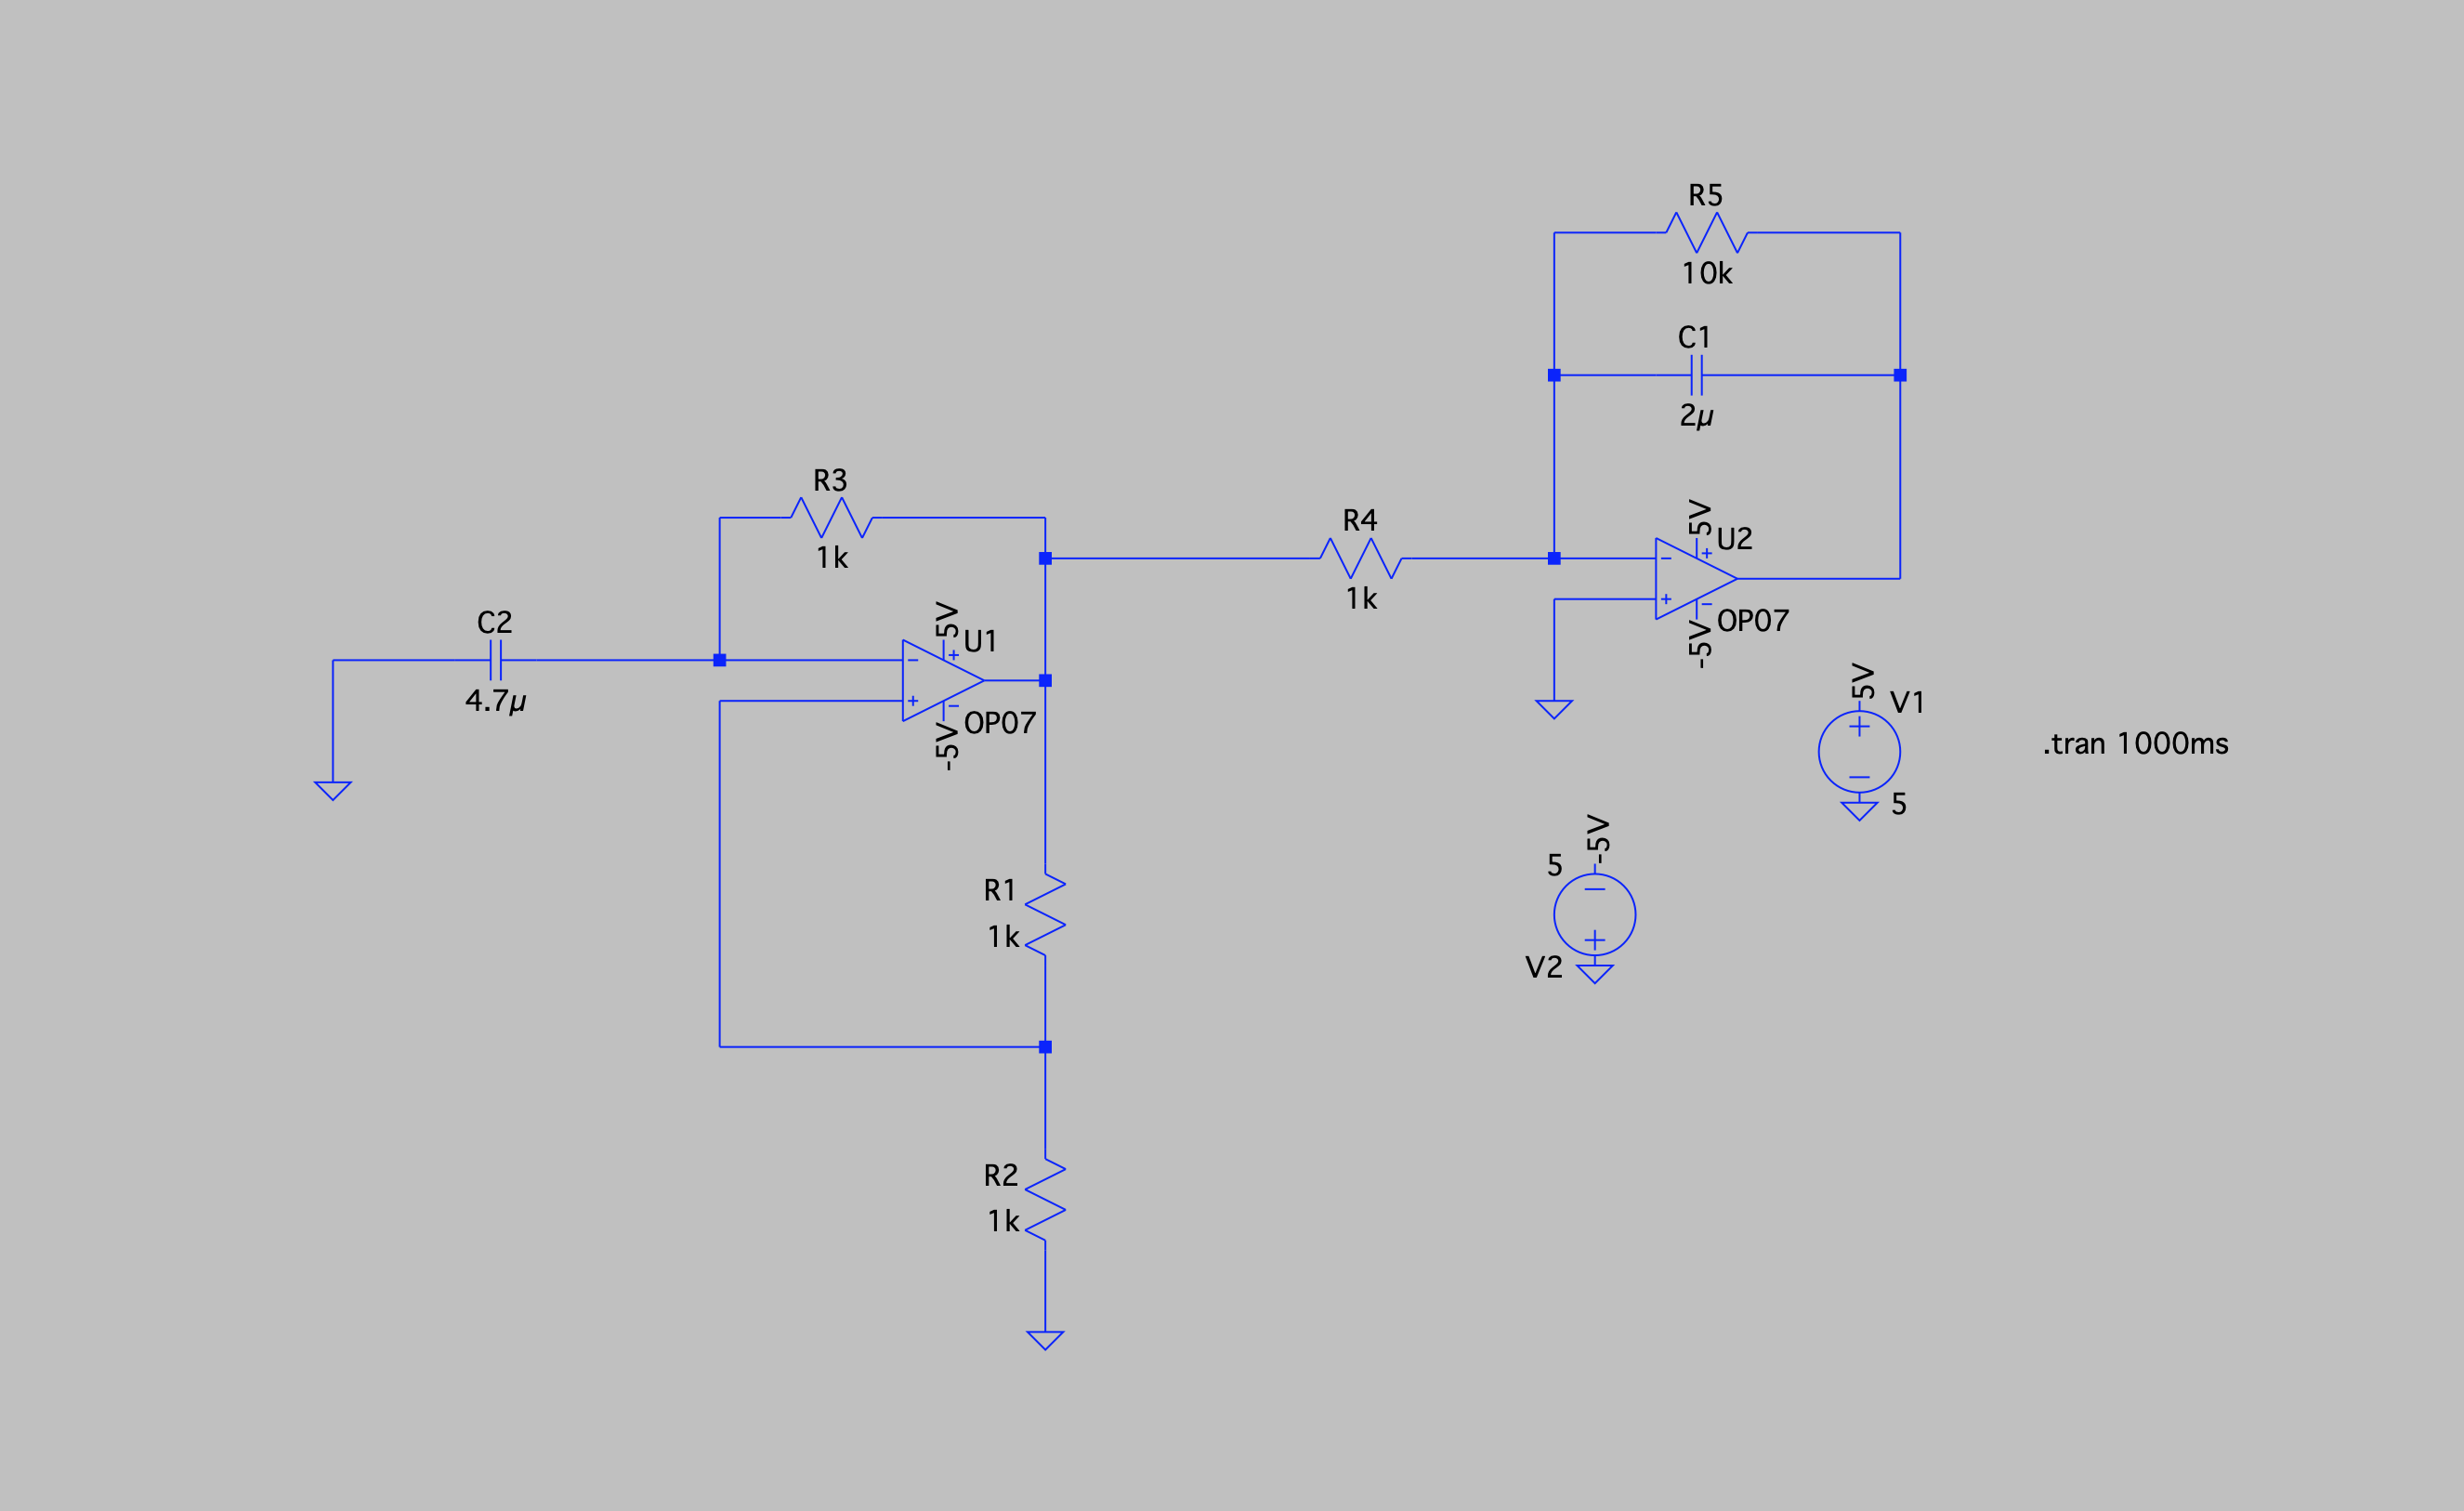
\includegraphics[width=0.5\textwidth]{../Img/E3Ckt.png}
  \caption{Circuit Diagram}
  \label{fig:image}
  \end{figure}

  \vspace*{\fill} % Fills the page with space to ensure that the content stays on a new page
  \newpage

  \subsection{Output:} 
    \begin{figure}[h!]
        \centering
        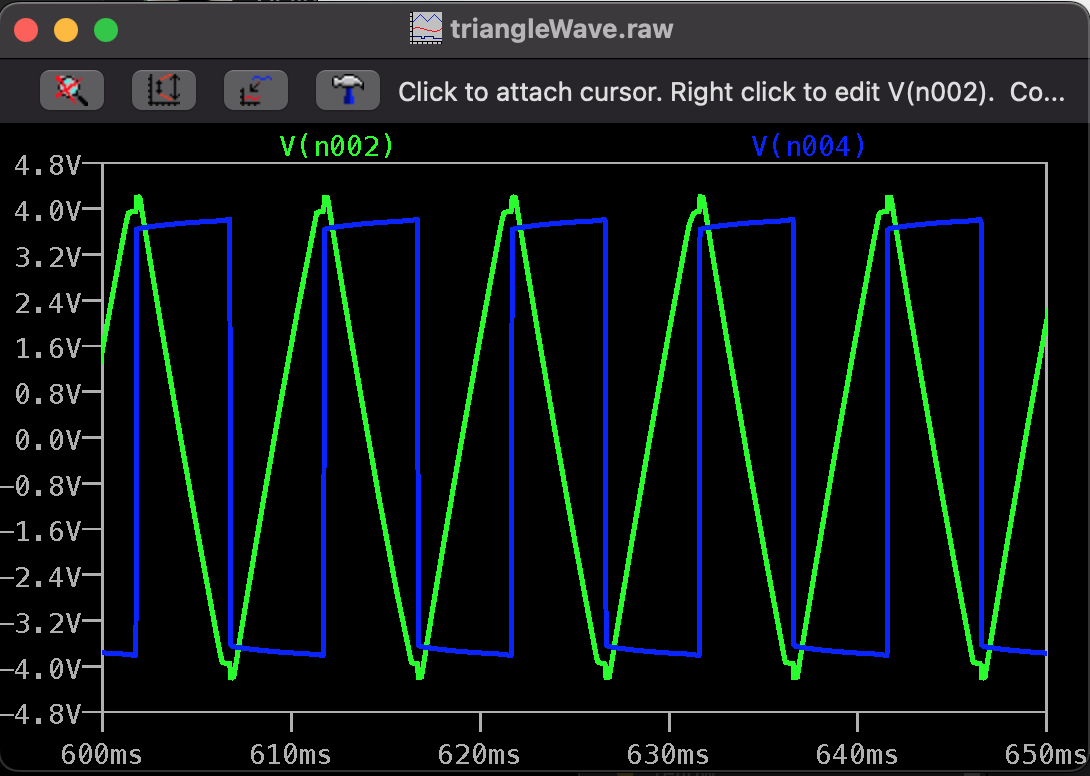
\includegraphics[width=0.8\textwidth]{../Img/E3OP.png}
        \caption{Output waveform from LTSpice}
    \end{figure}

  \vspace{0.3cm}

  \subsection{Conclusion:} 
    \hspace{20pt}Designed a Triangular and Square wave generator using OP Amps and verified the workings.

  \newpage

\section{Experiment 4}

  \subsection{Aim:}
    \hspace{20pt}Building a KHN filter and Verifying the AC output

  \vspace{0.3cm} % Adjust spacing between sections

  \subsection{Software Used:} 
    \hspace{20pt}LTSpice

  \vspace{0.3cm}

  \subsection{Design Parameters:}
    \begin{itemize}
        \item Opertaional Amplifier 0P07
    \end{itemize}

  \vspace{0.3cm}

  \subsection{Theory:} 
    \begin{itemize}
        \item \textbf{Function:} The KHN (Kerwin-Huelsman-Newcomb) filter is an active filter used to implement second-order filters like low-pass, high-pass, band-pass, and notch filters with precise control over frequency and quality factor.
        \item \textbf{Structure:} It consists of operational amplifiers, resistors, and capacitors arranged in a feedback configuration, allowing independent adjustment of gain, frequency, and quality factor.
        \item \textbf{Uses:} KHN filters are widely used in signal processing for filtering specific frequency bands with high accuracy, such as in audio processing and communication systems.
    \end{itemize}

  \vspace{0.3cm}

  \subsection{Circuit Diagram:} 
    \begin{figure}[htbp]
    \centering
      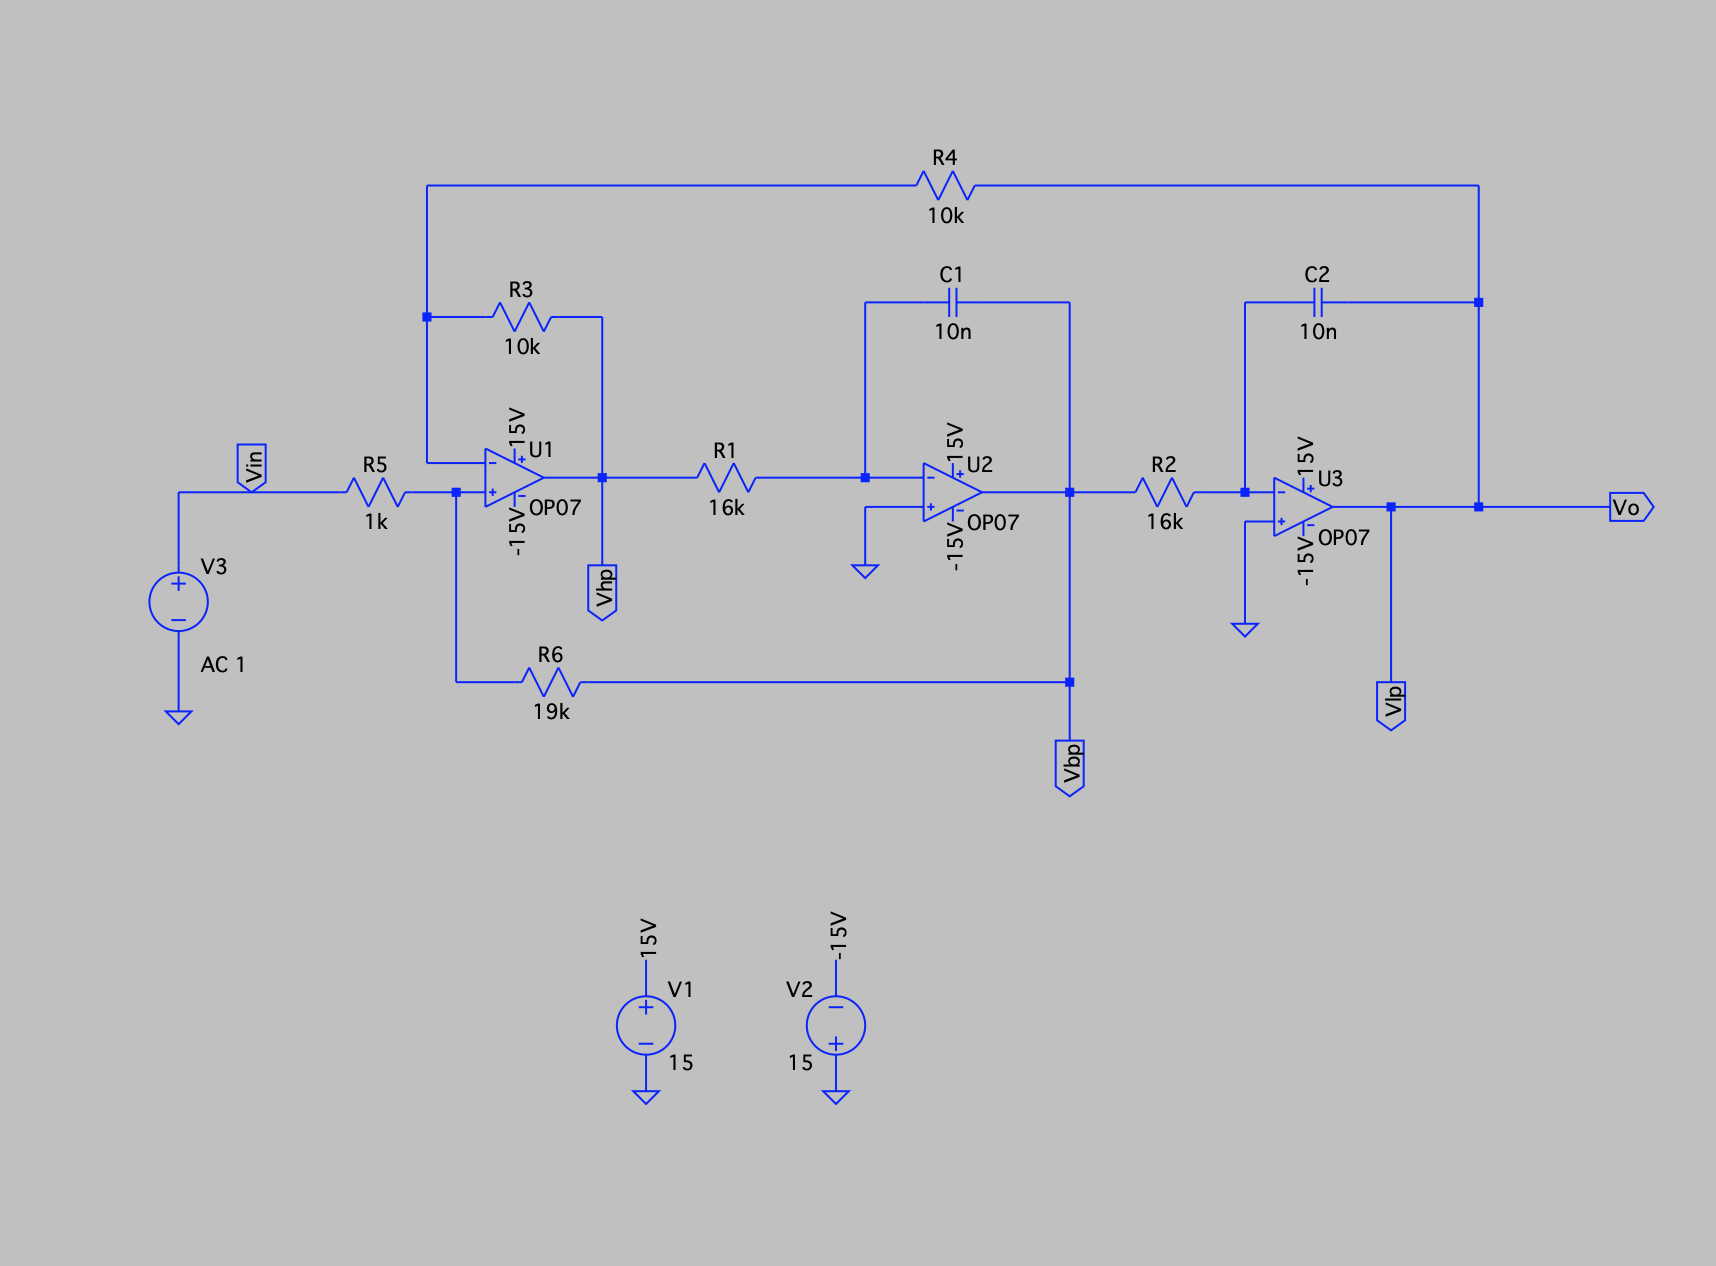
\includegraphics[width=0.5\textwidth]{../Img/E4Ckt}
    \caption{Circuit Diagram}
    \label{fig:image}
    \end{figure}

    \vspace*{\fill} % Fills the page with space to ensure that the content stays on a new page
    \newpage

  \subsection{Output:} 
    \begin{figure}[h!]
        \centering
        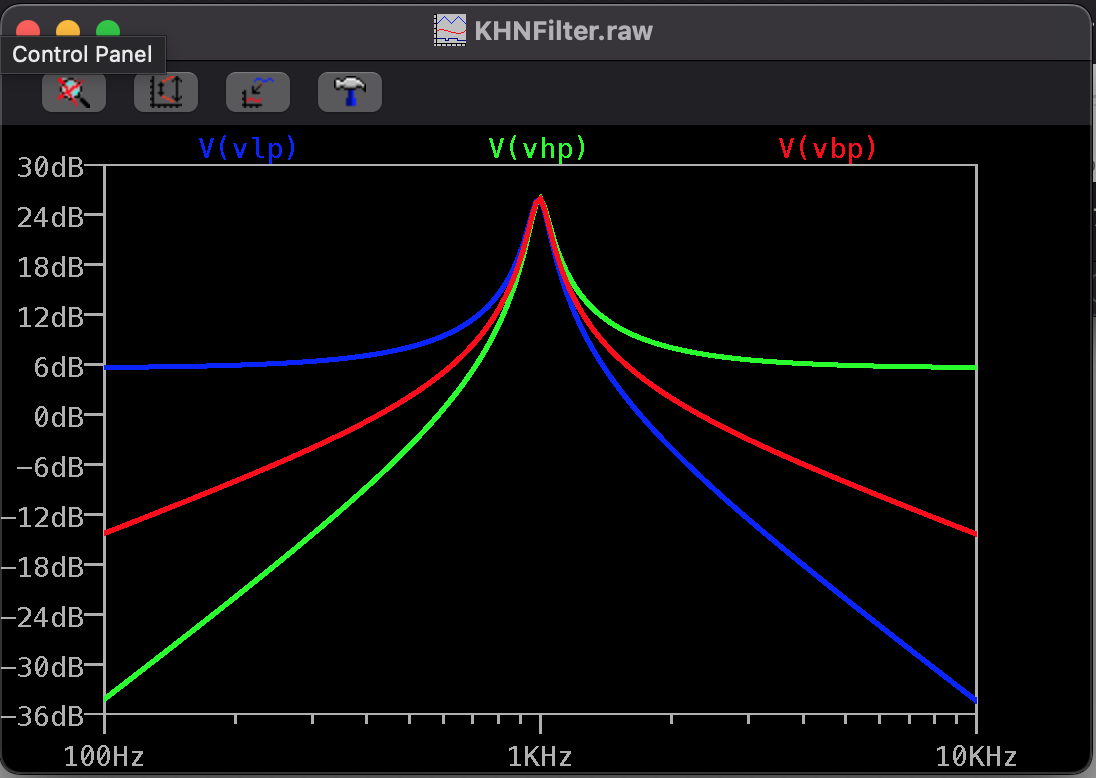
\includegraphics[width=0.8\textwidth]{../Img/E4Op}
        \caption{Output waveform from LTSpice}
    \end{figure}

  \vspace{0.3cm}

  \subsection{Conclusion:} 
    \hspace{20pt}Built a KHN filter and verified its AC output.

  \newpage

\section{Experiment 5}

\subsection*{Aim:}
  \hspace{20pt}To assemble and study the different feedback circuits using IC-741. The four configurations shown in the figure below are:
  \begin{enumerate}
      \item Voltage series feedback amplifier (VCVS)
      \item Voltage shunt feedback amplifier (CCVS)
      \item Current series feedback amplifier (VCCS)
      \item Current shunt feedback amplifier (CCCS)
  \end{enumerate}

  \vspace{0.3cm}

\subsection*{Software Used:}
  \hspace{20pt}\href{https://www.analog.com/en/design-center/design-tools-and-calculators/ltspice-simulator.html}{LTSpice}
  \vspace{0.3cm}

\subsection*{Design Parameters:}
  \hspace{20pt}\begin{itemize}
      \item Operational Amplifier OP07
  \end{itemize}
  \vspace{0.3cm}

\subsection*{Theory:}
  \hspace{20pt}Feedback circuits are essential in electronic systems, particularly in amplifiers, as they influence the performance, stability, and linearity of the system. Feedback refers to the process of taking a portion of the output signal and returning it to the input. Depending on how the feedback is applied, it can have different effects on the circuit's behavior. Here's a more detailed explanation of the four types of feedback circuits:

  \subsubsection*{1. Voltage Series Feedback (Voltage-Controlled Voltage Source - VCVS)}
    \textbf{Concept:} In this configuration, a portion of the output voltage is fed back in series with the input voltage.\\
    \newline
    \textbf{Effect:} This type of feedback reduces the gain of the amplifier but improves its linearity, bandwidth, and stability. It also increases the input impedance, making it easier to drive the circuit with a signal source.\\
    \newline
    \textbf{Applications:} Used in voltage amplifiers where maintaining a stable voltage gain is crucial.\\

  \subsubsection*{2. Voltage Shunt Feedback (Current-Controlled Voltage Source - CCVS)}
    \textbf{Concept:} Here, the output voltage is fed back in parallel (shunt) to the input.\\
    \newline
    \textbf{Effect:} This configuration lowers the input impedance and can increase the bandwidth of the amplifier. It helps to stabilize the gain and improve the linearity of the circuit.\\
    \newline
    \textbf{Applications:} Commonly used in transconductance amplifiers where the output voltage is regulated by the input current.\\

  \subsubsection*{3. Current Series Feedback (Voltage-Controlled Current Source - VCCS)}
    \textbf{Concept:} In this configuration, a portion of the output current is fed back in series with the input voltage.\\
    \newline
    \textbf{Effect:} This feedback reduces the input current and increases the input impedance, helping in stabilizing the current gain and improving the circuit's performance in terms of bandwidth and distortion.\\
    \newline
    \textbf{Applications:} Often used in current amplifiers where the output current needs to be controlled by the input voltage.\\

  \subsubsection*{4. Current Shunt Feedback (Current-Controlled Current Source - CCCS)}
    \textbf{Concept:} The output current is fed back in parallel (shunt) to the input.\\
    \newline
    \textbf{Effect:} This type of feedback decreases the output impedance and stabilizes the current gain. It also improves the linearity and reduces distortion in the amplifier.\\
    \newline
    \textbf{Applications:} Used in circuits requiring precise current control, such as in transimpedance amplifiers.\\

  \subsection*{General Benefits of Feedback Circuits:}
    \begin{itemize}
        \item \textbf{Stability:} Feedback reduces the effect of component variations and external disturbances, making the circuit more stable.
        \item \textbf{Linearity:} It improves the linearity of the amplifier, reducing distortion in the output signal.
        \item \textbf{Bandwidth:} Feedback can increase the bandwidth of the amplifier, allowing it to work effectively over a wider range of frequencies.
        \item \textbf{Impedance Control:} It allows designers to tailor the input and output impedance of the amplifier to suit specific applications.
    \end{itemize}

  Understanding these feedback mechanisms is crucial for designing and analyzing amplifiers that perform reliably in various electronic systems.

  \vspace{0.3cm}

  \subsection{Circuit Diagram:} 
    \begin{figure}[h]
        \centering
        \begin{minipage}{0.45\textwidth}
            \centering
            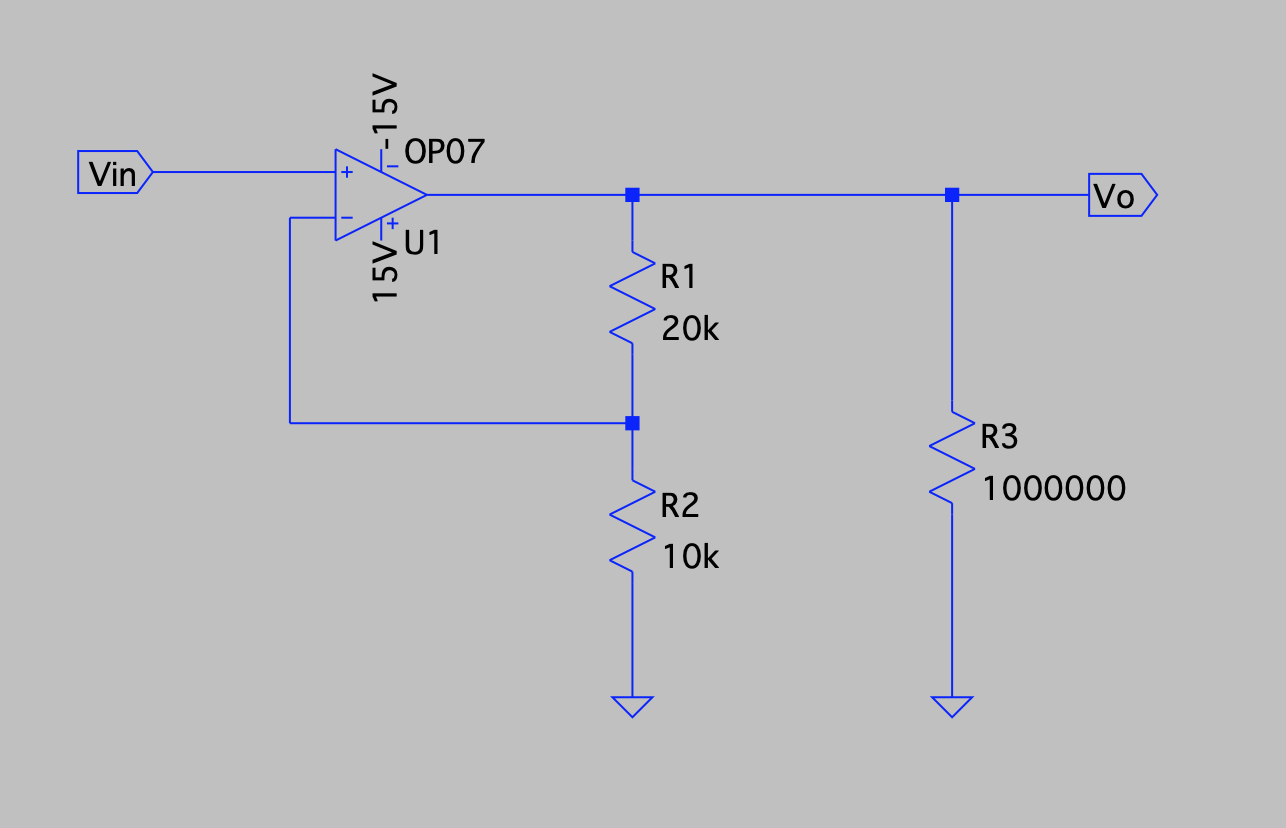
\includegraphics[width=\linewidth]{../Img/E5VCVS}
            \caption{Voltage Controlled Voltage Source}
        \end{minipage}
        \hfill
        \begin{minipage}{0.45\textwidth}
            \centering
            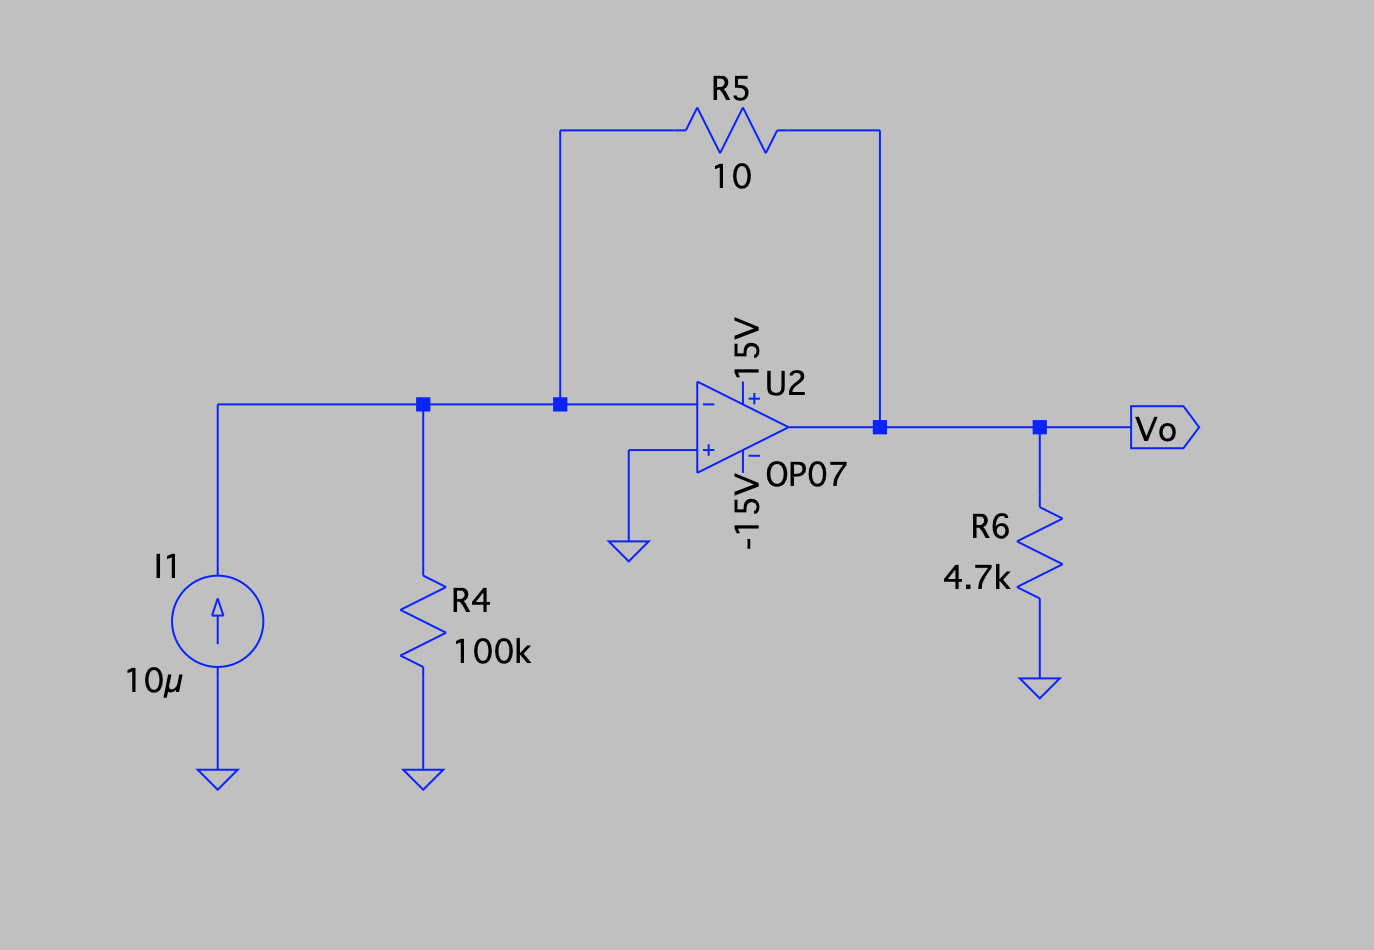
\includegraphics[width=\linewidth]{../Img/E5CCVS}
            \caption{Current Controlled Voltage Source}
        \end{minipage}
        
        \vspace{6cm}
        
        \begin{minipage}{0.45\textwidth}
            \centering
            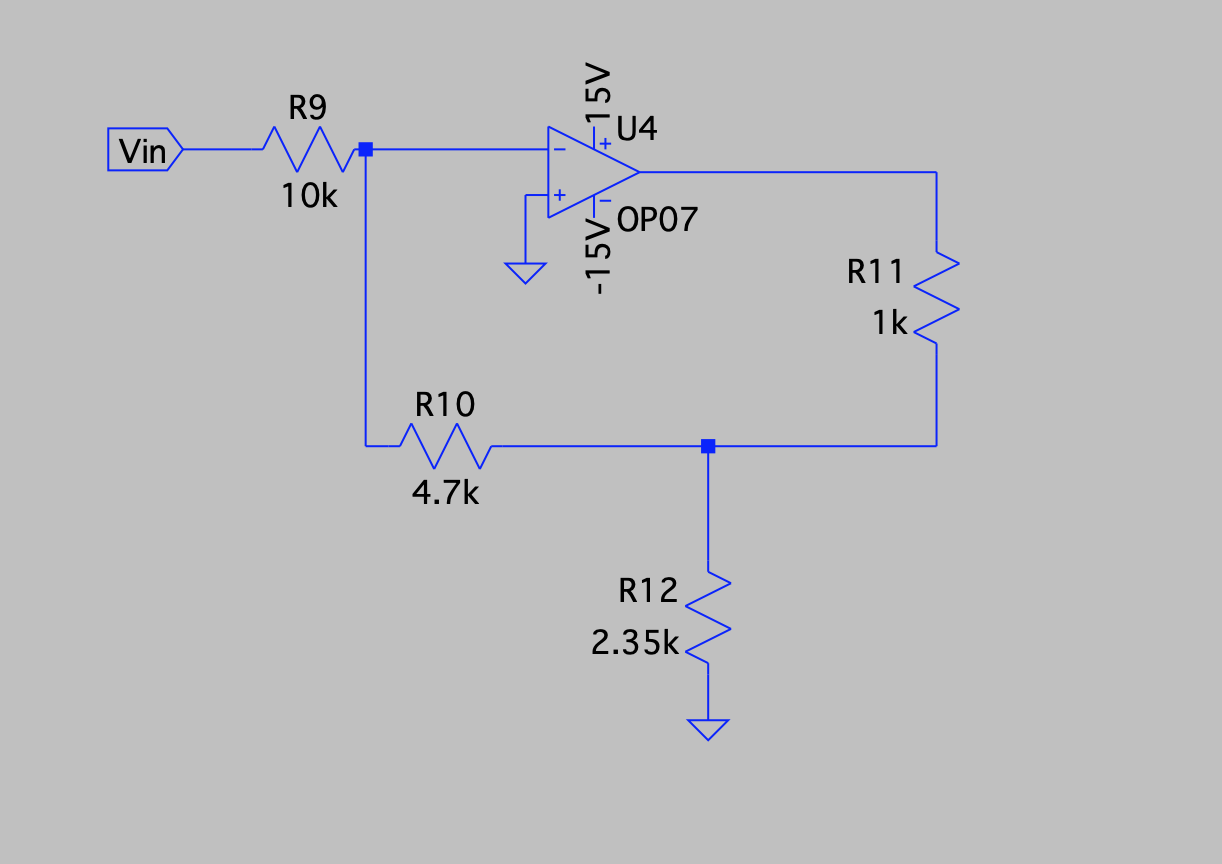
\includegraphics[width=\linewidth]{../Img/E5CCCS}
            \caption{Current Controlled Current Source}
        \end{minipage}
        \hfill
        \begin{minipage}{0.45\textwidth}
            \centering
            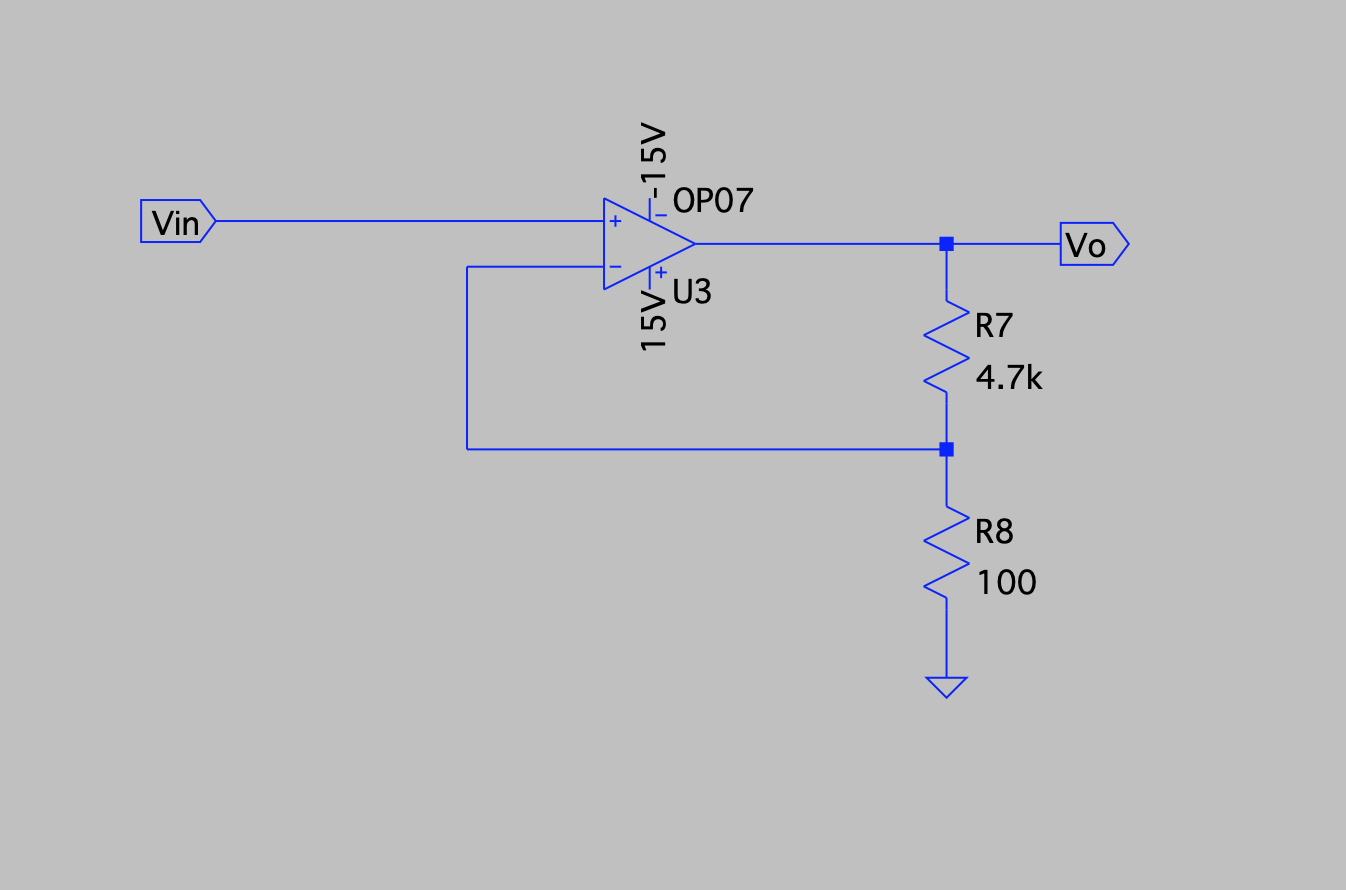
\includegraphics[width=\linewidth]{../Img/E5VCCS}
            \caption{Voltage Controlled Current Source}
        \end{minipage}
    \end{figure}

    \vspace*{\fill} % Fills the page with space to ensure that the content stays on a new page
    \newpage

  \subsection{Output:} 
    \begin{figure}[h]
        \centering
        \begin{minipage}{0.45\textwidth}
            \centering
            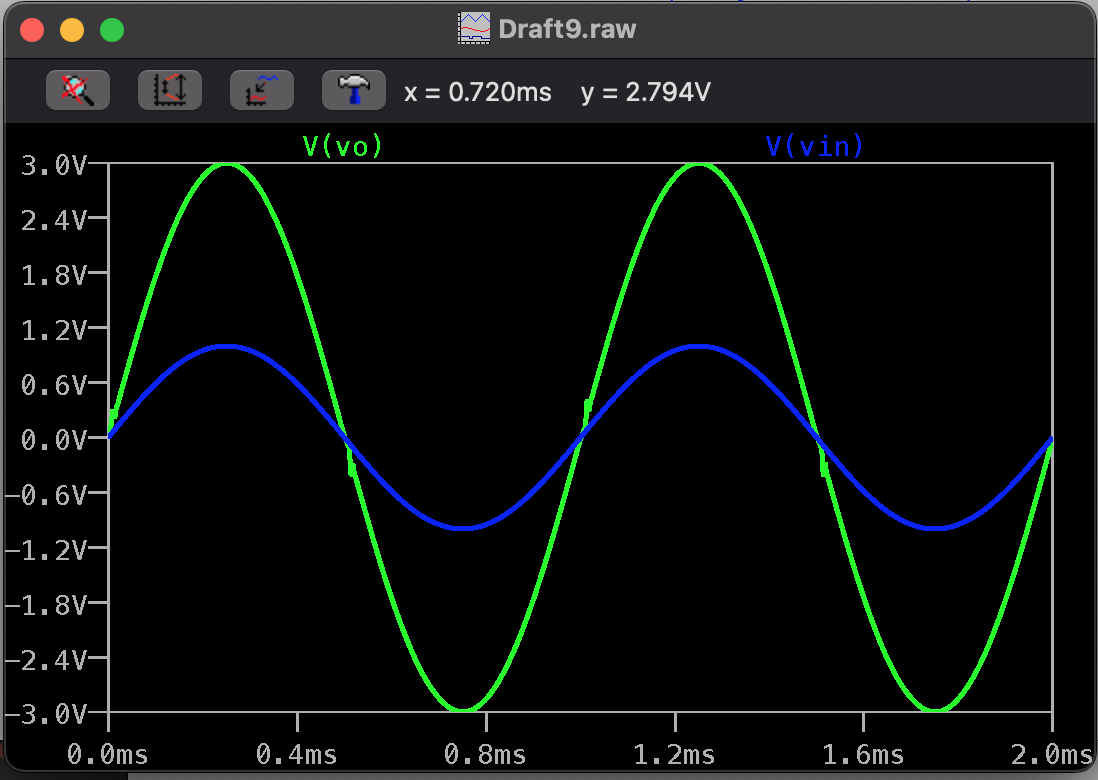
\includegraphics[width=\linewidth]{../Img/E5OpVCVS}
            \caption{Voltage Controlled Voltage Source Output}
        \end{minipage}
        \hfill
        \begin{minipage}{0.45\textwidth}
            \centering
            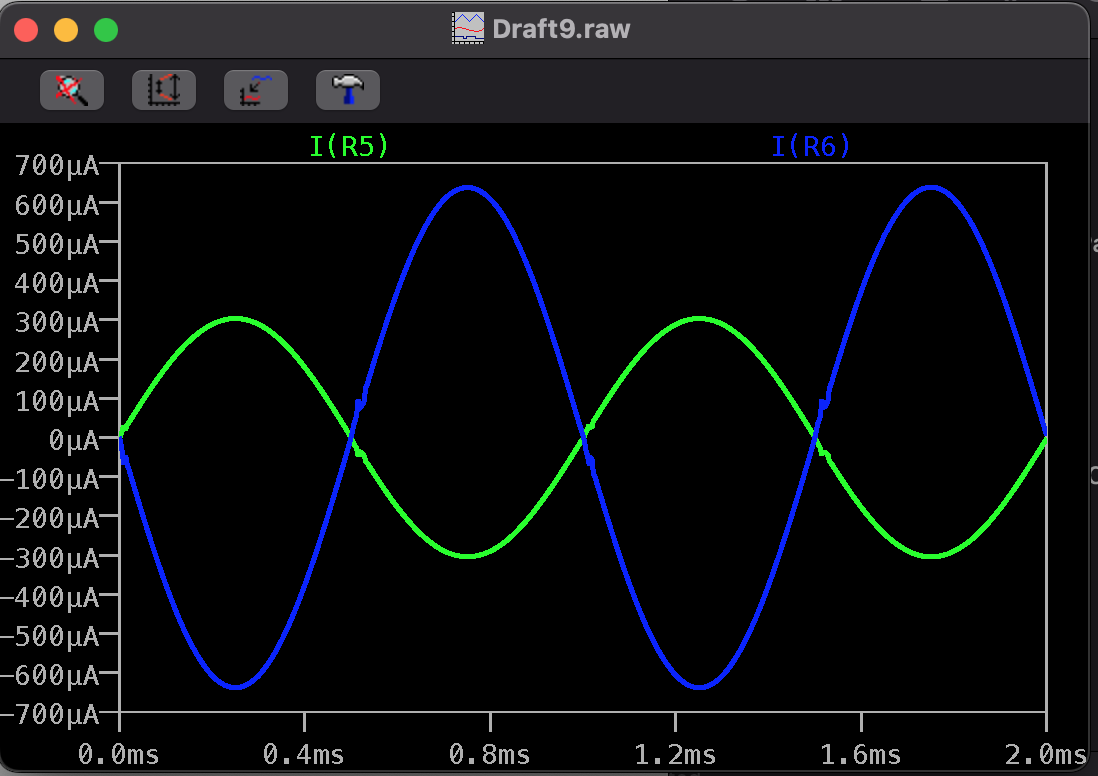
\includegraphics[width=\linewidth]{../Img/E5OpCCVS}
            \caption{Current Controlled Voltage Source Output}
        \end{minipage}
        
        \vspace{0.5cm}
        
        \begin{minipage}{0.45\textwidth}
            \centering
            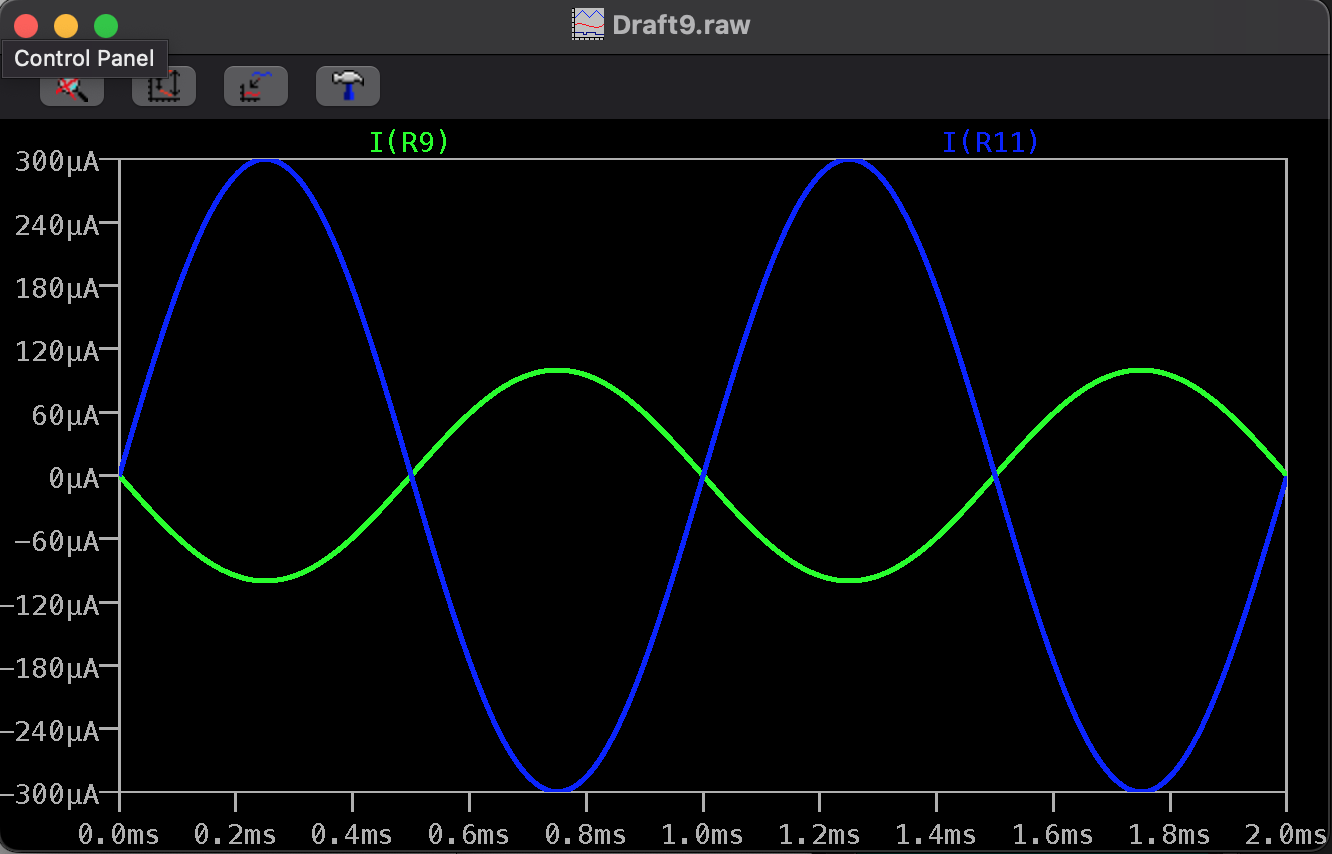
\includegraphics[width=\linewidth]{../Img/E5OpCCCS}
            \caption{Current Controlled Current Source Output}
        \end{minipage}
        \hfill
        \begin{minipage}{0.45\textwidth}
            \centering
            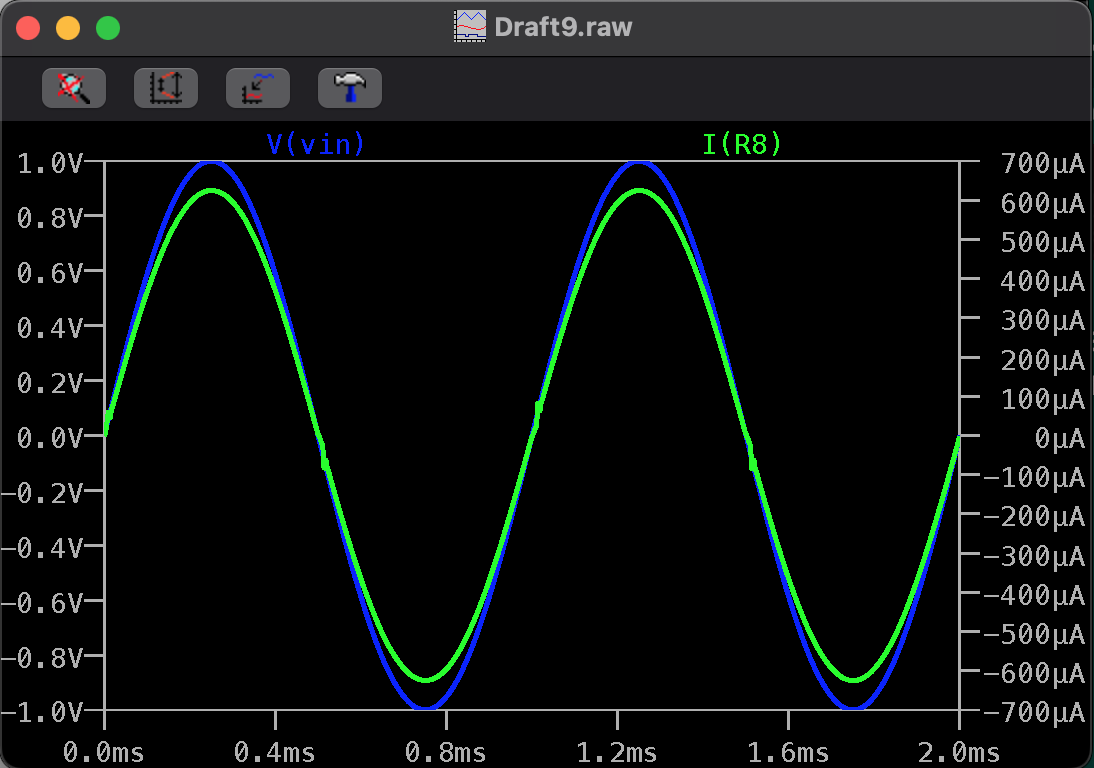
\includegraphics[width=\linewidth]{../Img/E5OpVCCS}
            \caption{Voltage Controlled Current Source Output}
        \end{minipage}
    \end{figure}

  \vspace{0.3cm}

  \subsection{Conclusion:} 
    \hspace{20pt}Built different types of Feedback amplifiers and verified their gain expressions.

  \newpage

\end{document}
